\documentclass[14pt,aspectratio=169,hyperref={pdftex,unicode},xcolor=dvipsnames]{beamer}
\usepackage[english,russian]{babel}
\usepackage[utf8x]{inputenc}
\usepackage[T2A]{fontenc}
\usepackage{cmap}
\usepackage{paratype}
\usepackage{minted} % для примеров кода (требует параметра -shell-escape)

\usetheme{metropolis}
\usefonttheme[]{professionalfonts}  % запрещаем beamer'у перезаписывать мат. шрифты
\metroset{numbering=fraction}
\metroset{subsectionpage=progressbar}

\setbeamercolor{frametitle}{fg=black}
\setbeamertemplate{frametitle}
{
 \vspace{3mm}\insertframetitle\par
}
\setbeamertemplate{title separator}{}
\setbeamertemplate{footnote separator}{}


\usebackgroundtemplate{
\includegraphics[width=\paperwidth,height=\paperheight]{./common/background_white.jpg}}

\logo{\vspace{-1.2cm}
\includegraphics[width=6mm]{./common/short-v.pdf}\hspace*{1.08\textwidth}}

\institute
{
  \begin{columns}
    \begin{column}{1.5cm}
    
\includegraphics[height=15mm,keepaspectratio]{./common/math-cs.pdf}
    \end{column}
    \begin{column}{4cm}
          Факультет математики и компьютерных наук СПбГУ
    \end{column}
  \end{columns}
}


\begin{document}

\begin{frame}[plain]

\begin{center}
\textbf{Иван Добрынин}

{\Large\textbf{Разработка комплекса информационных систем для проведения соревнований и тренировок по спортивному программированию в формате дуэли}}

Выпускная квалификационная работа

{\small Научный руководитель: Д.\,С.\,Шалымов}

10.06.2026
\end{center}

\begin{columns}
\begin{column}{1cm}

\includegraphics[height=15mm,keepaspectratio]{./common/math-cs.pdf}
\end{column}
\begin{column}{10cm}
    \small
        Факультет математики и~компьютерных наук СПбГУ\\
        Программа <<Современное программирование>>
\end{column}
\end{columns}

\end{frame}

\begin{frame}
\frametitle{Введение в предметную область}

\begin{center}
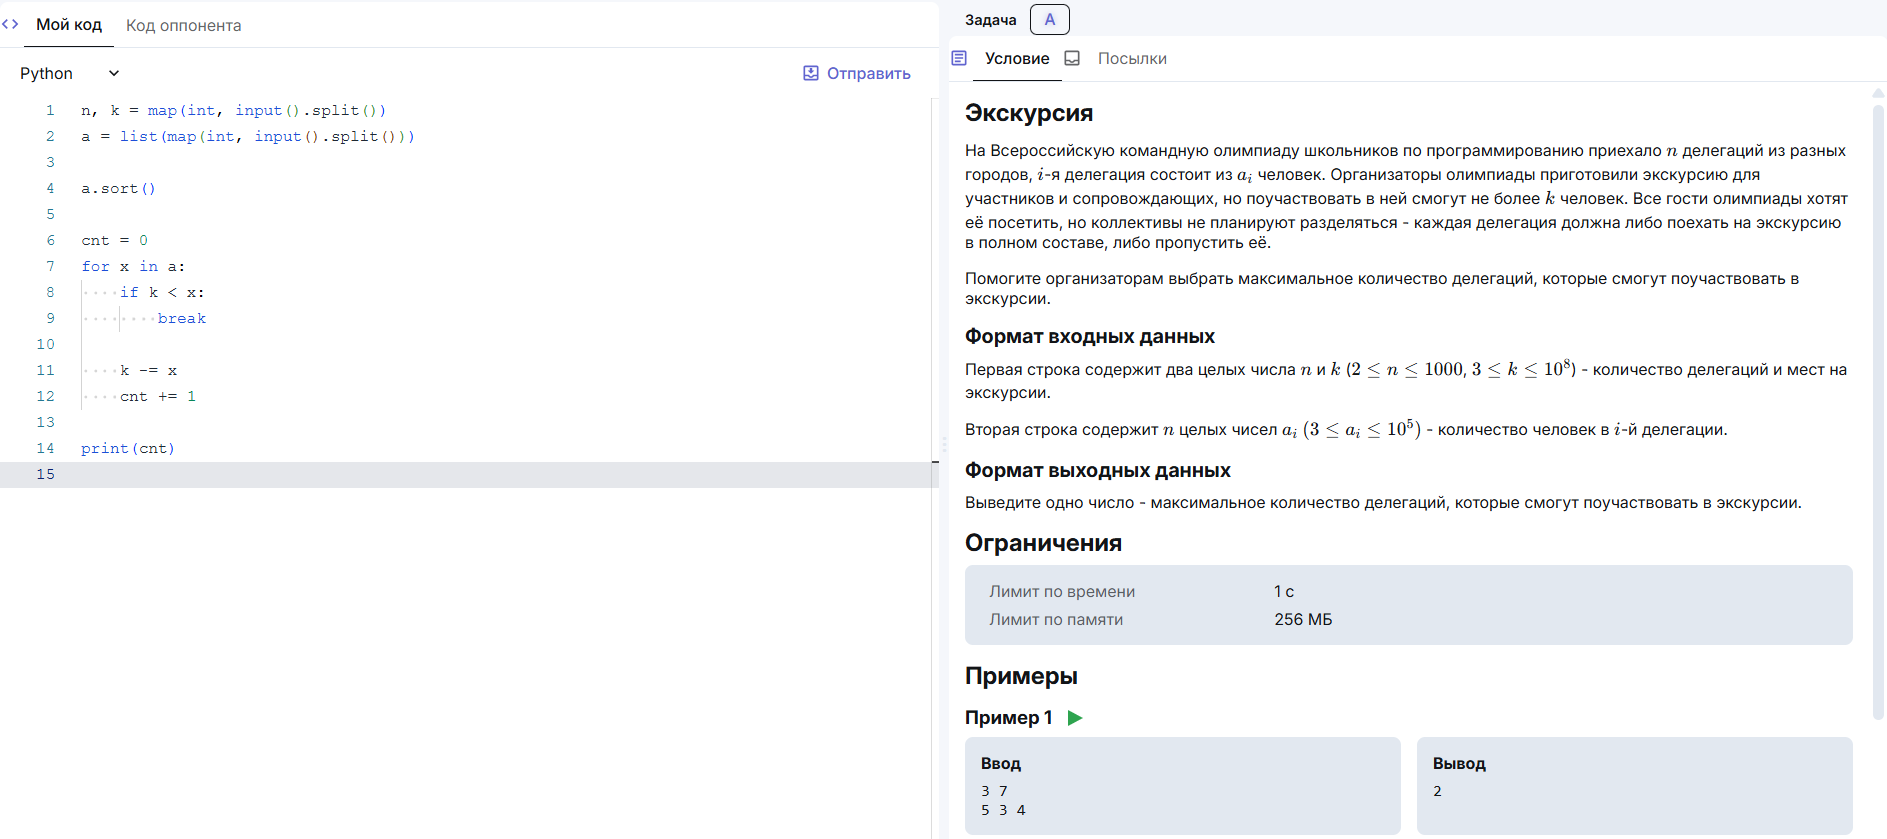
\includegraphics[width=13cm]{images/duel.png}
\end{center}

\end{frame}

\begin{frame}
\frametitle{Сравнение существующих платформ}

\small
\centering
\begin{tabular}{lccc}
    Критерий & 
\includegraphics[height=0.5cm]{images/codeforces_logo.png} & 
\includegraphics[height=0.5cm]{images/leetcode_logo.png} & 
\includegraphics[height=0.5cm]{images/codebattle_logo.png} \\
\hline\hline
    Проведение дуэлей & $-$ & $-$ & $+$ \\
    Разная структура турниров & $-$ & $-$ & $\pm$ \\
    Использование своих задач & $+$ & $\pm$ & $\pm$ \\
    Нестандартные типы задач & $-$ & $-$ & $-$ \\
    Анализ поведения участников & $-$ & $-$ & $-$ \\
\end{tabular}

\end{frame}

\begin{frame}
\frametitle{Постановка задачи}

\small
\begin{enumerate}
\item Спроектировать архитектуру системы, позволяющую проводить дуэли по спортивному программированию.
\item Разработать масштабируемую тестирующую систему для автоматической проверки решений пользователей с параллельным исполнением и эффективным использованием вычислительных ресурсов.
\item Написать и протестировать код всех компонентов системы и взаимодействие между ними.
\item Исследовать подход к обнаружению подозрительных участников на основе анализа поведения в сессии дуэли.
\end{enumerate}

\end{frame}

\begin{frame}{Микросервисная архитектура системы}

\begin{center}

\includegraphics[width=14cm]{images/architecture.png}
\end{center}

\end{frame}

\begin{frame}{Схема асинхронного процесса тестирования}

\begin{center}
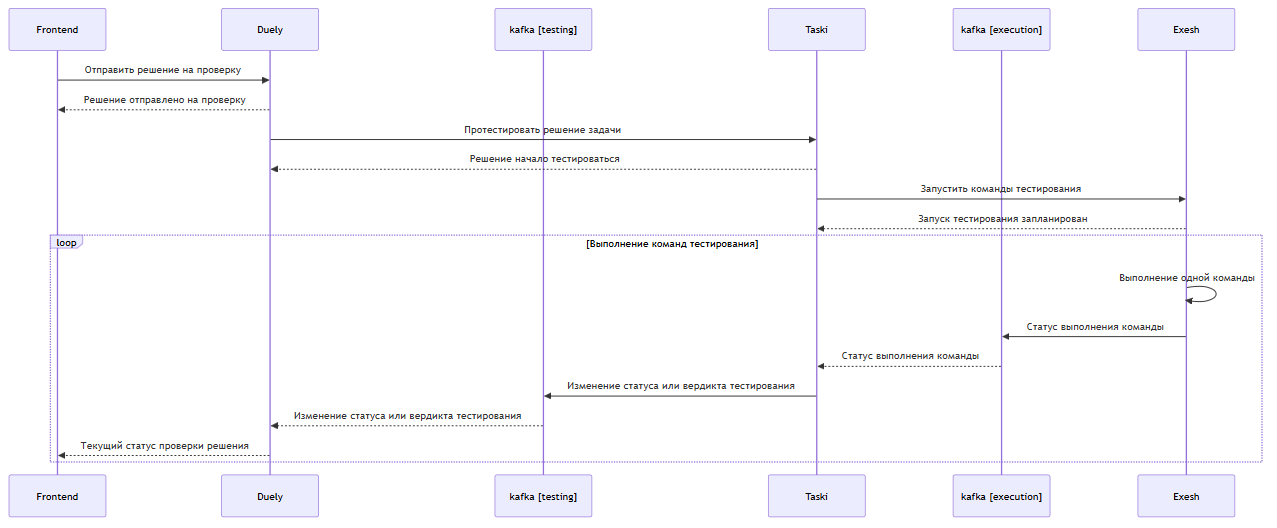
\includegraphics[width=14cm]{images/pipeline_testing.png}
\end{center}

\end{frame}

\begin{frame}{Распределённое исполнение графа команд}

\begin{center}
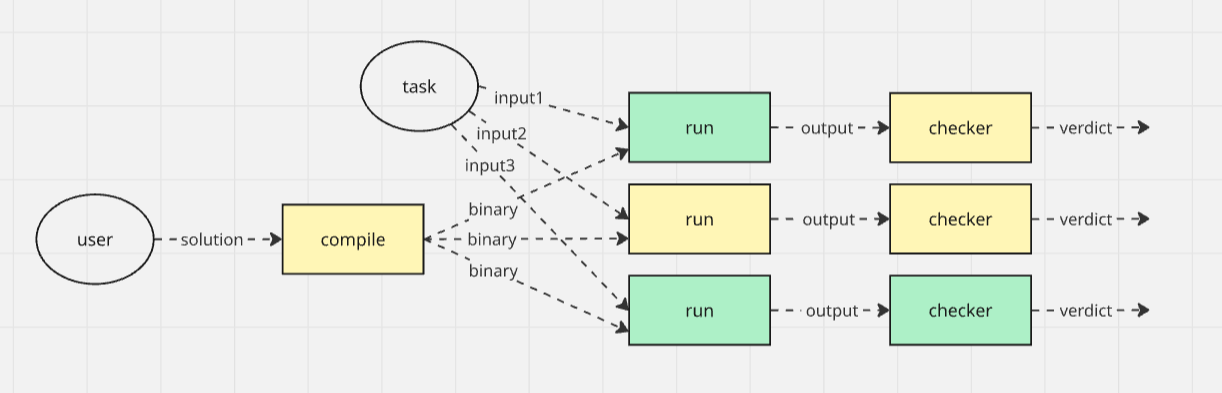
\includegraphics[width=14cm]{images/execution_graph.png}
\end{center}

\end{frame}

\begin{frame}{Архитектура Exesh на основе модели оркестрации}

\begin{center}
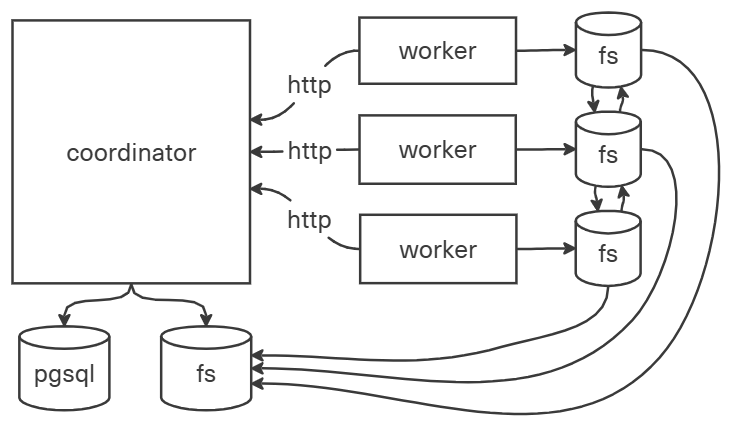
\includegraphics[width=10cm]{images/architecture_exesh.png}
\end{center}

\end{frame}

\begin{frame}{Хранение и передача файлов между компонентами системы}

\small
    \textbf{filestorage} --- библиотека на Go:
    \begin{itemize}
    \item Абстракция над файловой системой.
    \item Кэширование файлов для повторного использования.
    \item Передача файлов между компонентами в сжатом виде.
    \item Автоматическая очистка неиспользуемых файлов.
    \end{itemize}

\end{frame}

\begin{frame}{Честное распределение ресурсов для одновременного исполнения набора Execution}

\begin{center}
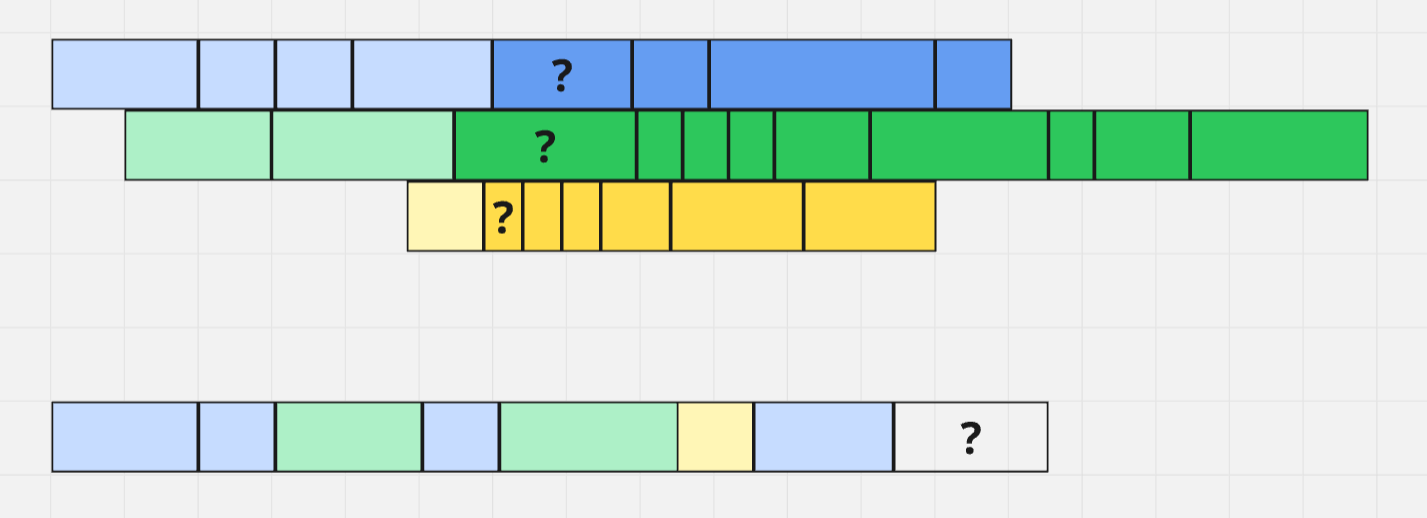
\includegraphics[width=12cm]{images/executions_problem.png}
\end{center}

\end{frame}

\begin{frame}{Честное распределение ресурсов для одновременного исполнения набора Execution}

\small
    \begin{equation*}\label{eq:priority}
    priority(T) = \frac{T - T_{start}}{T_{total}} + \alpha \cdot \frac{T_{total} - T_{done}}{T_{total}}
    \end{equation*}

    \begin{itemize}
    \item $T_{start}$ --- время начала исполнения.
    \item $T_{total}$ --- общая ожидаемая продолжительность исполнения.
    \item $T_{done}$ --- общая ожидаемая продолжительность уже исполненной части.
    \item $\alpha$ --- определяет влияние реальной и ожидаемой оставшейся продолжительности исполнения.
    \end{itemize}

\end{frame}

\begin{frame}{Распределение Jobs по исполнителям для эффективной утилизации ресурсов}

\begin{center}
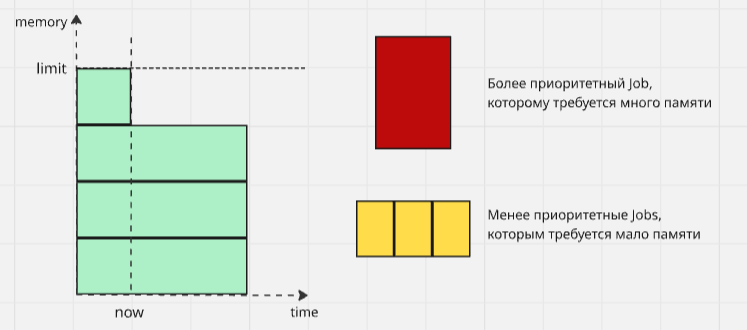
\includegraphics[width=10cm]{images/jobs_problem.png}
\end{center}

\end{frame}

\begin{frame}{Распределение Jobs по исполнителям для эффективной утилизации ресурсов}

\begin{center}
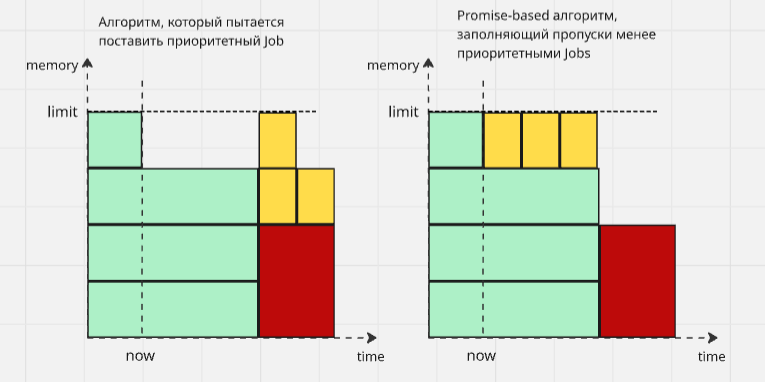
\includegraphics[width=10cm]{images/jobs_algorithm.png}
\end{center}

\end{frame}

\begin{frame}{Безопасный запуск пользовательского кода в изолированном окружении}

\small
    \textbf{isolate} --- утилита на C от ioi:
    \begin{itemize}
    \item Изоляция процессов для предотвращения доступа к ресурсам других процессов.
    \item Ограничение ресурсов, доступных для выполнения кода.
    \item Запрет взаимодействия с сетью.
    \item Лёгкий вес и высокая производительность.
    \end{itemize}

\end{frame}

\begin{frame}{Анализ подозрительности поведения участника при участии в дуэли}

\begin{center}
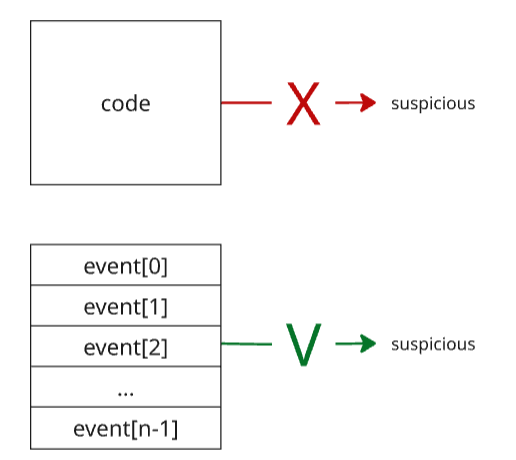
\includegraphics[width=7cm]{images/analyzer_intro.png}
\end{center}

\end{frame}

\begin{frame}{Анализ подозрительности поведения участника при участии в дуэли}

\begin{center}
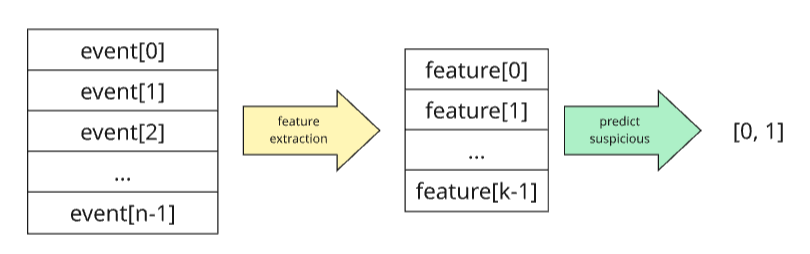
\includegraphics[width=12cm]{images/analyzer_pipeline.png}
\end{center}

\end{frame}

\begin{frame}{Анализ подозрительности поведения участника при участии в дуэли}

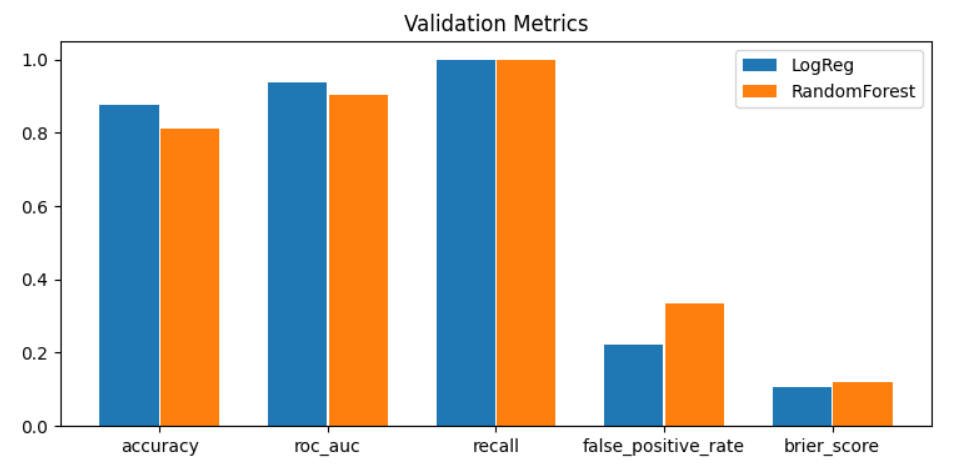
\includegraphics[height=4.25cm]{images/analyzer_validation_metrics.png}
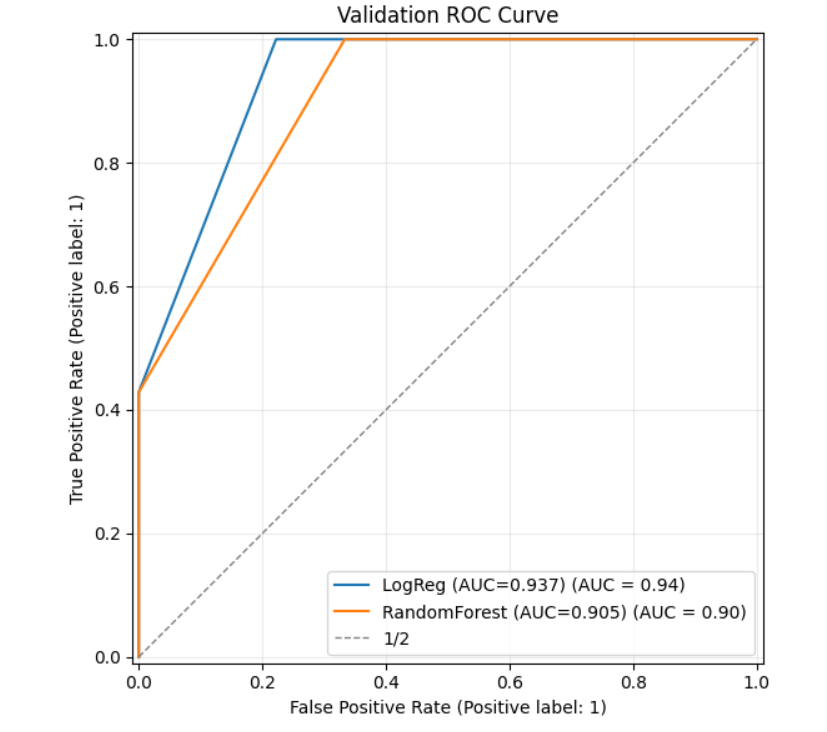
\includegraphics[height=4.25cm]{images/analyzer_roc_curve.png}

\end{frame}

\begin{frame}{Настройка правил проведения дуэлей и турниров}

\begin{center}
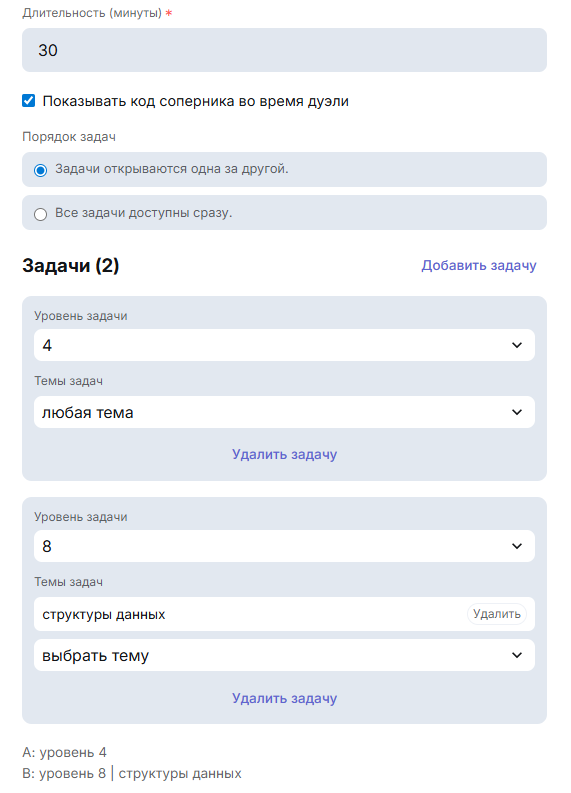
\includegraphics[width=4cm]{images/duel_configuration.png}
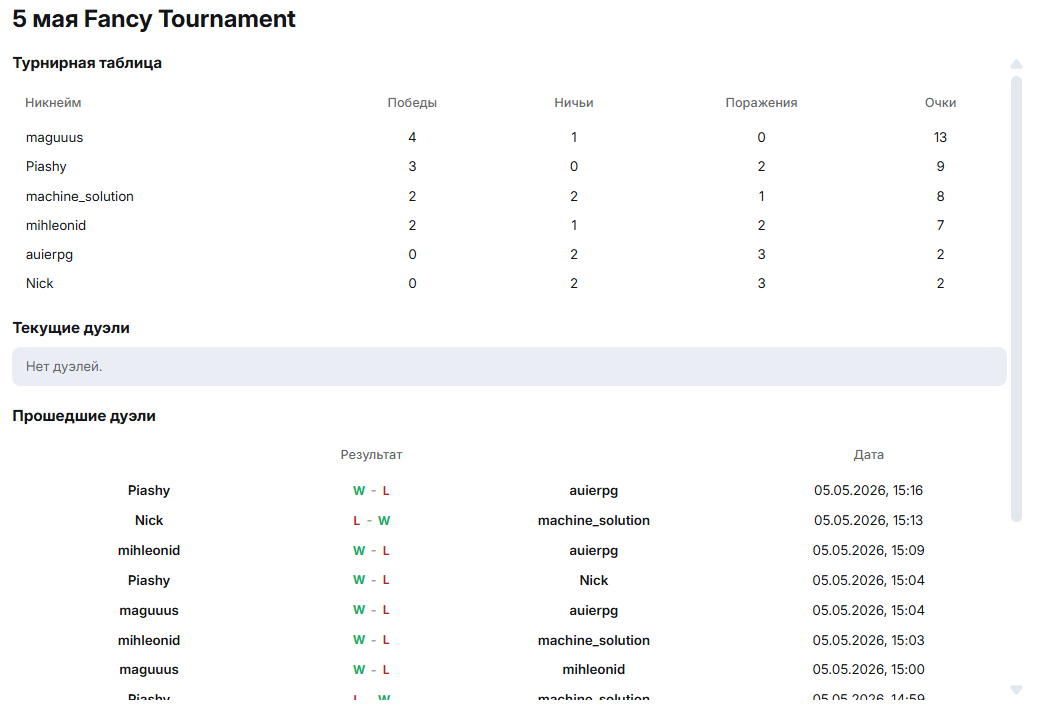
\includegraphics[width=8cm]{images/tournament.png}
\end{center}

\end{frame}

\begin{frame}
\frametitle{Результаты работы}

\begin{enumerate}
\item Разработан комплекс информационных систем для проведения соревнований и тренировок по спортивному программированию в формате дуэли.
\item Реализована распределённая тестирующая система с планированием выделения ресурсов и поддержкой масштабирования.
\item Исследован подход к анализу подозрительности поведения пользователя во время дуэли.
\end{enumerate}

\end{frame}

\end{document}